%
\chapter{Satelitski sistemi za določanje lastnega položaja}
\label{Ch:LastPolSat} % Always give a unique label
% use \chaptermark{}
% to alter or adjust the chapter heading in the running head
%https://en.wikibooks.org/wiki/LaTeX/Floats,_Figures_and_Captions
%https://www.sharelatex.com/learn/Positioning_images_and_tables

%%%%%%%%%%%%%%%%%%%%%%%%%%
% Kaj je WGS-84? Kaj je elipsoid? http://www.znanostnacesti.si/blog/kako-visok-je-triglav.aspx
%%%%%%%%%%%%%%%%%%%%%%%%%%

%\begin{figure*}[!ht]
%	\begin{center}
%		\includegraphics[height=4cm]{Predavanja/05_SatLastPolozaj/figs/Trilateracija.png}  
%		%\hspace*{1.0cm}
%		\caption{Prikaz trilateracije s pomočjo merjenja časov potovanja signalov.}
%		\label{Fig_Trilateracija}
%	\end{center}
%\end{figure*}

%	\centering
%	\includegraphics[height=5cm]{Predavanja/Uvod/figs/Sun_Compass_d.jpg}
%	\hspace*{1.0cm}
%	\includegraphics[height=5cm]{Predavanja/Uvod/figs/RekonstrukcijaVikingSunCompass_s.png}\\
%	\vspace*{0.25cm}
%	\includegraphics[height=5cm]{Predavanja/Uvod/figs/Kristal-SonceVInIzOPticneOsi_.png}
%	\includegraphics[height=5cm]{Predavanja/Uvod/figs/VikingSunstoneCompass.jpg}
%	\caption{\textbf{Sončni kompasi} (zgoraj) Disk iz Uunartoka, Grenlandija, najden v samostanu iz 11. stoletja, naj bi predstavljal izsek sončnega kompasa Vikingov. Rekonstrukcija: \href{DOI: 10.1098/rspa.2016.0171}{\textit{Dénes Száz et al., Eötvös Loránd Tudományegyetem, Madžarska}} (spodaj) Ko so srednjeveški pomorščaki optično os prozornega dvolomnega monokristala kalcita z Islandije usmerili natančno v Sonce, so dobili na zaslonu namesto dveh pik le eno, s čimer so lahko določali smeri neba tudi v manj jasnih dneh. Rekonstrukcija: \href{http://www.livescience.com/16831-viking-sunstone-crystal-compass.html}{\textit{Guy Ropars, Université de Rennes, Francija.}}}


\begin{wrapfigure}{r}{0.5\textwidth}
	\vspace{-60pt}
	\begin{center}
		\includegraphics[width=0.48\textwidth]{Predavanja/05_SatLastPolozaj/figs/SkicaECEF.png}
	\end{center}
	\vspace{-10pt}
	\caption{Zemlja, prikazana v obliki zemeljskega sestava (ECEF), z izhodiščem v masnem središču Zemlje, z oznakami osi kartezičnega sistema ($\vec{x}^{\textrm{zem}}$,$\vec{y}^{\textrm{zem}}$,$\vec{z}^{\textrm{zem}}$) in z označeno smerjo vrtenja, ekvatorjem ($\varphi$ = 0\degree) in ničelnim poldnevnikom ($\lambda$ = 0\degree).}
	\label{Fig_PrikazECEF}
	\vspace{130pt}
\end{wrapfigure}



Zaradi praktičnih razlogov si Zemljo predstavljamo (modeliramo) kot rotacijski elipsoid.
Razmerje dolžin polosi Zemlje je na sliki \ref{Fig_PrikazECEF} zaradi nazornosti narisano veliko večje, kot je v naravi, saj iz  \href{http://nssdc.gsfc.nasa.gov/planetary/factsheet/earthfact.html}{podatkov}
vemo, da znaša povprečni ekvatorialni polmer Zemlje 6378,137 km ($a$), polarni pa 6356,752 km ($b$). Sploščenost Zemlje $f$ (ang. flatness) je definirana kot razlika razmerja do enakosti obeh polmerov. Ponavadi se podaja z inverzno vrednostjo $1/f = 1 - a/b$, kar iz zapisanih podatkov znaša $1/297,25284$, približno 0,3\%. Idealna krogla ima inverzno sploščenost enako $0,0000$. 

\begin{wrapfigure}{r}{0.5\textwidth}%[!ht]
	\vspace{-120pt}
	\begin{center}
		\includegraphics[width=4cm]{Predavanja/05_SatLastPolozaj/figs/2009-02-28-Skica-LokGeod.png}
	\end{center}
	\vspace{-10pt}
	\caption{Prikaz lokalnega geodetskega levosučnega koordinatnega sistema \textit{north-east-up} (NEU) z oznakami osi po geodetski literaturi. }
	\label{Fig_LokGeodet}
	\vspace{-40pt}
\end{wrapfigure}

Ker v izračunih za določanje položaja Zemljo modeliramo z geoidom, ki se najbolj prilega navigacijskim potrebam, so bolj znani $1/f$ geoidov. Za geoid WGS-84, ki ga uporablja sistem GPS, je $1/f$ natančno $1/298,257223563$, za GRS-80 pa $1/298,257222100882711$. 


S postajami v vesolju dosegamo podobne učinke kot s postajami na Zemlji. Ker so satelitske postaje na znanih položajih in med seboj so zelo natančno časovno usklajene, objektom lahko določamo razdalje do postaj. S povezovanjem večih rešitev določamo položaj objektom natančneje in v za opazovalca najbolj primernem koordinatnem sistemu.



\begin{figure}[!ht]
	\centering
	\vspace{-15pt}
	\includegraphics[width=1.0\textwidth]{Predavanja/05_SatLastPolozaj/figs/geoid.png} 
	\vspace{-10pt}
	\caption{Ko Zemljo nadomestimo z vrtenino najbolj prilegajočega se elipsoida WGS-84, opazimo odstopanja (m), ker površina Zemlje ni ravna. Borre, \textit{geoid.m}.}
	\label{Fig_PrikazGeoid}
\end{figure}

Na sliki \ref{Fig_LokGeodet} vidimo nastanek razlike v geografski širini ($\varphi \rightarrow \varphi^\prime$) v točki dotikališča z vodoravno ravnino lokalnega geodetskega sistema. Razlika med širinama v sistemih nastaja, ker pravokotnica na površino elipsoida in zveznica dotikališča s težiščem Zemlje nista vzporedni.


Bodoči pomorščaki morate ta pristop dobro proučiti. Kako? 

Postavite si preprosto vprašanje: Iz katerih podatkov sklepam, da sem na položaju, ki ga kaže navigacijska naprava ali iz katerih informacij sklepam, da plujem po tem kurzu? Odgovor mora biti znanstveno podprt, da mu pomorščak sme verjeti. Znanstveniki so ugotovili, da se dve napravi, ki delujeta na različnih principih, \textit{težko hkrati pokvarita}. Z veliko večjo verjetnostjo daje samo po ena napačne rezultate, kot obe naenkrat, še posebno, če so okoliščine neugodne samo za eno od njiju. Tudi to morate dobro proučiti in preizkušati.

%slabljenje: moč 250W po 20.000km pade na ...



Vsak satelit GNSS neprestano oddaja signale, ki dosežejo zemeljsko površje že zelo oslabljeni. S signali sateliti pošiljajo informacije o svojem pložaju in točnem času. Na Zemlji sprejemniki primerjajo čase v katerih so signale prejeli, s časom v katerih so sateliti signale oddali. Iz izmerjene in ocenjene razlike sprejemniki ocenjujejo oddaljenost do satelita v trenutku oddaje signala, glej sliko \ref{Fig_Trilateracija}). Z radionavigacijskimi satelitskimi sistemi določamo položaj s pomočjo določanja vsaj treh ocen razdalje, imenovanih psevdorazdalje. Oceni psevdorazdalje se zmanjša negotovost, ko v izračun vključijo še popravke zaradi okoliščin (relativnost, ionosfera, vesoljsko vreme, troposfera, večpotje, itd). 

Iz popravljenih razdalj do večih satelitov sprejemnik izračuna svoj položaj v prostoru. Postopek na splošno imenujemo trilateracija, ker izračunana koordinata sledi neposredno iz treh oddaljenosti (rešitev je presečišče krogel okoli položajev satelitov, glej sliko \ref{Fig_Trilateracija}). 
Za izračun položaja v prostoru mora v resnici sprejemnik dobivati podatke od vsaj štirih satelitov nad obzorjem. Sprejemnik namreč potrebuje še en satelit več nad obzorjem, kot če bi imel za meritve časa prihoda signala točno uro, zaradi neznanega odstopanja merilnika časa sprejemnika od točnega časa. Šele po določitvi tudi četrte psevdorazdalje pa je mogoč izračun odstopanja ure sprejemnika od ur satelitov in avtonomna določitev položaja sprejemnika v prostoru zemeljskega sestava.



Ničelni poldnevnik sestava WGS 84 je referenčni meridian (IERS), ki poteka 5,3 ločne sekunde oz. $ 102m $ vzhodno od Greenwich-kega meridiana, ki predstavlja geografsko dolžino Kraljevega observatorija \ref{fig:GreenwichRO}.

Središče Zemlje postavimo v središče koordinatnega sestava, os z je usmerjena v smeri vrtenja zemeljske osi. Ločimo dva sestava:
ECEF - Earth Centered Earth Fixed .. (zemeljski sestav) sestav glede na Zemljo mirujočih osi Zemlje, osi x in y ležita v ravnini zemeljskega ekvatorja ohranjata usmerjenost od središča Zemlje do točke na površini Zemlje: os x prebada krog, ki ga tvorita ekvator in geoid na dogovorjenem ničelnem meridianu (Conventional Zero Meridian), os y pa na $90^\circ$ vzhodnejšem meridianu.    
ECI - Earth Centered Inertial .. (astronomski sestav) sestav glede na Zemljo vrtečih se osi Zemlje, osi x in y v ravnini zemeljskega ekvatorja mirujeta glede na mirujoče vesolje, glede na zemeljski sestav pa se x in y vrtita.

%\begin{SCfigure}%[htb]
%	\centering
%	\caption{Zemlja, prikazana v obliki zemeljskega sestava, izhodišče v masnem središču Zemlje, z oznakami osi kartezičnega sistema ($\vec{x}^{\textrm{zem}}$,$\vec{y}^{\textrm{zem}}$,$\vec{z}^{\textrm{zem}}$) in z označeno smerjo vrtenja, ekvatorjem ($\varphi$ = 0\degree) in ničelnim poldnevnikom ($\lambda$ = 0\degree).}
%	\includegraphics[width=0.5\textwidth]{Predavanja/05_SatLastPolozaj/figs/SkicaECEF.png}  
%	\label{Fig_PrikazECEF}
%\end{SCfigure}





     

%\begin{figure}
%	\centering
%	\includegraphics[height=6cm]{Predavanja/05_SatLastPolozaj/figs/LastnostiGNSS.png}
%	\caption{Lastnosti določanj položaja, hitrosti in časa z GNSS.}
%	\label{fig:Gnss_Polozaj:GnssLastnosti}
%\end{figure}

%https://en.wikibooks.org/wiki/LaTeX/Floats,_Figures_and_Captions
%https://www.sharelatex.com/learn/Positioning_images_and_tables

Znanost utrjuje temelje tehnologijam in išče nove rešitve. Inženirji izdelujejo nove navigacijske ali merilne naprave, ki izpisujejo številske rezultate, \textit{katerim uporabnik \textbf{lahko} zaupa}. Če uporabnika iz povsem slepega zaupanja ne potegnejo navodila za uporabo, ga v razmislek prisilita ali nesrečen splet naravnih okoliščin ali celo namerno vplivanje na signale oz. podatke. Na lastni koži uporabnik spozna pomen besede \textbf{\textit{lahko}}, v skrbi za lastno preživetje ga začne zanimati pojem besede verjetnost. 
Kljub veliki tehnični izpopolnjenosti naprav, bodo okoliščine še vedno odločale ali bodo uporabljane naprave delovale v skladu z našimi pričakovanji ali ne slika \ref{fig:Gnss_Polozaj:GnssLastnosti}.

\vspace{10pt}

\begin{wrapfigure}{r}{0.5\textwidth}
	\vspace{-35pt}
	\begin{center}
		\includegraphics[width=0.4\textwidth]{Predavanja/05_SatLastPolozaj/figs/LastnostiGNSS.jpg}
	\end{center}
	\vspace{-15pt}
	\caption{Lastnosti določanj položaja, hitrosti in časa z GNSS.}
	\label{fig:Gnss_Polozaj:GnssLastnosti}
	\vspace{-10pt}
\end{wrapfigure}

\vspace{15pt}

 Občutek za realnost nam vračajo preizkusi zanesljivosti in integritete, ne pa točnost naprave, še manj natančnost. Točnost je podana z določenim zaupanjem. Zanesljivost in intergiteta pa določata ali mi v resnici vemo, da se naprava moti, ali dobimo znamenje, da naprava ne deluje v skladu z našimi pričakovanji.


%ship-img-master768.jpg

\begin{figure}
	\centering
	\includegraphics[height=5.5cm]{Predavanja/05_SatLastPolozaj/figs/DSC00285_merid.png}
	\hspace*{1.0cm}
	\includegraphics[height=5.5cm]{Predavanja/05_SatLastPolozaj/figs/20140923_160146.png}\\
	\vspace*{0.25cm}
	\caption{\textbf{Royal Observatory, Greenwich} (levo) V naravi. (desno) Na pametnem telefonu.}
	\label{fig:GreenwichRO}       % Give a unique label
\end{figure} 





   





\section{Kako sprejemnik GNSS določi položaj?}
\label{Gnss_Polozaj}



%ORBITAL INCLINATION: https://en.wikipedia.org/wiki/Orbital_inclination
%EQUATORIAL COORDINATE SYSTEM: https://en.wikipedia.org/wiki/Equatorial_coordinate_system
%VERTICAL DATUM TRANSFORMATION (geodetic datums): http://vdatum.noaa.gov/docs/datums.html#geodetic
%DOLŽINA DVIŽNEGA VOZLA: https://sl.wikipedia.org/wiki/Dol%C5%BEina_dvi%C5%BEnega_vozla
%PREGLED NEBESNIH KOORDINATNIH SISTEMOV: (https://sl.wikipedia.org/wiki/Nebesni_koordinatni_sistem) 
%	Pregled nebesnih koordinatnih sistemov
%	Ime koordinatnega sistema	Referenčna ravnina	Osnovna smer	Središče	Dolžina	Oznaka dolžine	Širina	Oznaka širine
%	horizontni					horizont	poldnevnik opazovalca	stojišče opazovalca	azimut	Az, A	altituda	Alt, α
%	ekvatorski					ekvator	pomladišče	središče Zemlje	deklinacija	δ, (Dec)	rektascenzija	α, (RA)
%	ekliptični					ekliptika	pomladišče	središče Zemlje	longituda	λ	latituda	β
%	galaktični					galaktična ravnina	središče Rimske ceste	središče Sonca	galaktična longituda	l	galaktična latituda	b
%	supergalaktični	supergalaktična ravnina	presečišče supergalaktične in galaktične ravnine	Rimska cesta	supergalaktična dolžina	SGL	supergalaktična širina	SGB 
%NOAA Space Weather Scales: http://www.swpc.noaa.gov/sites/default/files/images/NOAAscales.pdf
%GLOSSARY: http://www.swpc.noaa.gov/content/space-weather-glossary#geomagneticelements
%Lagrangian Point: https://en.wikipedia.org/wiki/Lagrangian_point#L1
%South Korea to build eLoran system after jamming incident: http://gpsworld.com/south-korea-to-build-eloran-system-after-jamming-incident/
%TECHNICAL ARTICLE • MAY/JUNE 2016 Listening for RF Noise: http://www.insidegnss.com/node/4955 
%Nationwide Differential Global Positioning System (NDGPS): https://www.federalregister.gov/documents/2016/07/05/2016-15886/nationwide-differential-global-positioning-system-ndgps
%Aviation Safety Knowledge: http://www.skybrary.aero/index.php/Main_Page
%GNSS Performances: http://www.navipedia.net/index.php/GNSS_Performances
%The Future of Everything: Making Sense of the Sensor Revolution from a Telecoms Perspective: http://iot.ieee.org/newsletter/july-2016/the-future-of-everything-making-sense-of-the-sensor-revolution-from-a-telecoms-perspective


%JAMMING http://www.kbradar.by/en/products/radioelektronnaya-borba/peredatchiki-i-kompleksy-pomekh-navigatsionnoy-apparature-potrebiteley-sistem-gps-i-glonass/114/

\begin{wrapfigure}{r}{0.5\textwidth}
	\vspace{-20pt}
	\begin{center}
		\includegraphics[width=0.48\textwidth]{Predavanja/05_SatLastPolozaj/figs/Trilateracija.png}
	\end{center}
	\vspace{-10pt}
	\caption{Prikaz trilateracije položaja sprejemnika (rdeča pika), izvedene s pomočjo merjenja časov potovanja signalov od satelitov do sprejemnika.}
	\label{Fig_Trilateracija}
	\vspace{-20pt}
\end{wrapfigure}

Išče presečišča krogel, ki jih dobimo s časi potovanja posameznih signalov s satelitov do sprejemnika oz. s prekrivanjem izsekov hiperboloidov, dobljenih iz razlik časov potovanja večih parov satelitov do enega sprejemnika. 



\vspace{80pt}
Koliko satelitov kroži nad nami? \href{www.trimble.com/gnssplanningonline/#/SkyPlot}{\textit{Firefox na nebu}} \href{http://www.trimble.com/gnssplanningonline/#/WorldView}{\textit{Firefox svetovno}}  

\href{http://gpsworld.com/the-almanac/}{\textit{almanah vseh satelitskih navigacijskih tehnologij}}  

Uradne informacije koliko Galileo satelitov trenutno deluje: \href{https://www.gsc-europa.eu/system-status/Constellation-Information}{\textit{Firefox GSC}}  

V kakšnih okoliščinah se bodo signali s satelitov razširjali? \href{http://www.trimble.com/gnssplanningonline/#/IonoMap}{\textit{trimble iono karta}} 
\href{http://www.trimble.com/gnssplanningonline/#/IonoInformation}{\textit{trimble iono info}} 

%\cite{monograph}.

\subsection{Triki v sprejemniku}
\label{Gnss_Polozaj:Triki}


\begin{figure}
	\centering
	\includegraphics[height=12cm]{Predavanja/05_SatLastPolozaj/figs/dn20202691.jpg}
	\caption{Princip določanj položaja s sateliti poznamo že od Loran-a.}
	\label{fig:Gnss_Polozaj:GnssLorPrinc}
\end{figure}

%http://gpsinformation.net/main/gpspower.htm
%How much POWER do the GPS Satellites output on the 1575mhz L1 frequency?
%One of our anonomous newgroup readers gave this correct answer..
%In the frequency allocation filing the L1 C/A power is listed as 25.6 Watts.  The Antenna gain is listed at 13 dBi.  Thus, based on the frequency allocation  filing, the power would be about 500 Watts (27 dBW).
%Now, the free space path loss from 21000 km is about 182 dB.  Take the 500 Watts (27 dBW) and subtract the free space path loss (27 - 182) and you get  -155 dBW. The end of life spec is -160 dBW, which leaves a 5 dB margin.
%And if you really get into it, you'll discover ALL of the following represent the same approximate signal strength for GPS on the face of the earth (m stands for milliwatts and m2 stands for meters squared):
%-160 dBW, -130 dBm, -135 dBW/m2, -105 dBm/m2, -223 dBW/Hz, -163 dBW/MHz, -193 dBm/Hz, -198 dBW/m2/Hz, -138 dBW/m2/MHz
%Once you figure out why they're all the same, you're well on your way to understanding power, power density, and power flux density as it relates to GPS. For those that wish to quibble, I am assuming an even distribution of 
%power density over a 2 MHz C/A bandwidth.



\begin{equation}
\vec{a}\times\vec{b}=\vec{c}
\end{equation}

\subsubsection{11.000 letna rekonstrukcija števila Sončevih peg}
%https://en.wikipedia.org/wiki/Sunspot#/media/File:Sunspots_11000_years.svg

Sončeve pege so začasni pojavi v fotosferi Sonca, ki izgledajo temnejši kot okolica. Pege so območja z nižjo površinsko temperaturo, ker pretok magnetnega polja zavira konvekcijo toplote in plazme iz notranjosti Sonca. Število Sončevih peg sledi približno 11 let dolgemu ciklu Sončeve dejavnosti.

\begin{figure}
	\centering
	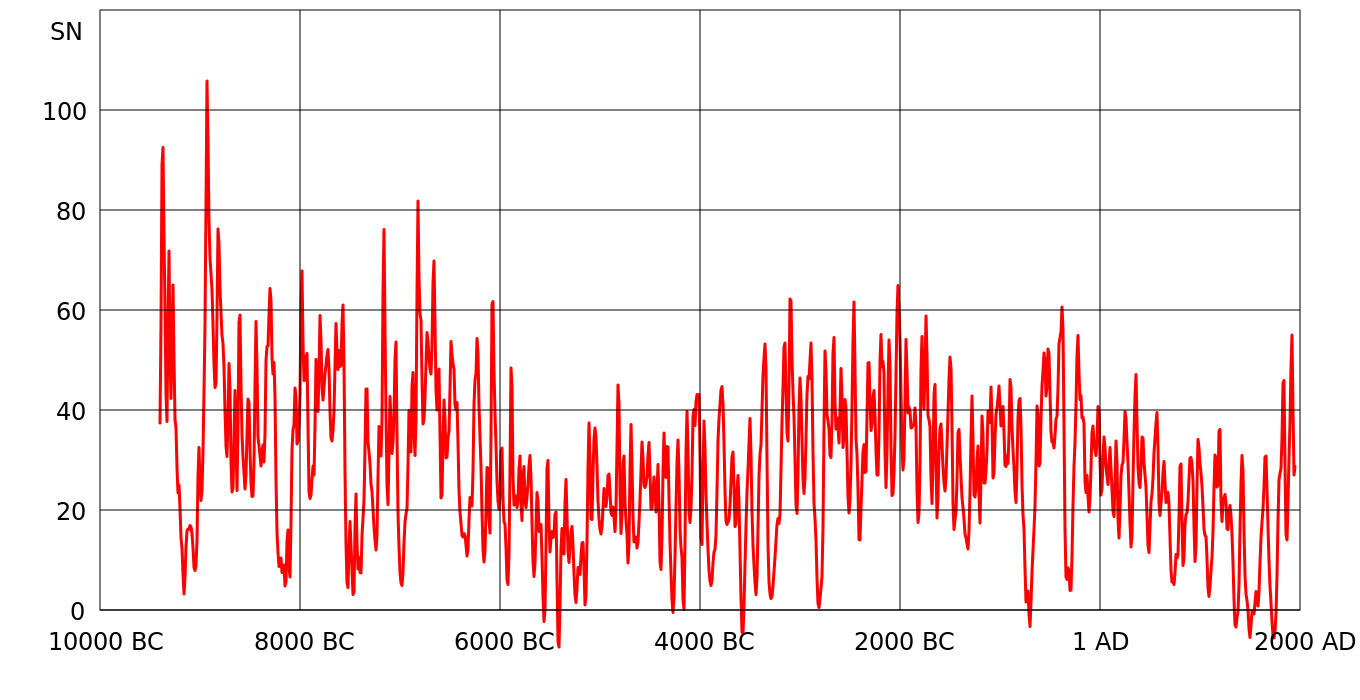
\includegraphics[height=7cm]{Predavanja/05_SatLastPolozaj/figs/Sunspots_11000_years.png}
	\caption{Od 1750 naprej štejemo število peg na Soncu, dotlej je število ocenjeno posredno iz \textit{geoloških koledarjev}.}
	\label{fig:Gnss_Polozaj:11tisocLetSN}
\end{figure}



\paragraph{Paragraph Heading} %
Your text goes here.

\subparagraph{Subparagraph Heading.} Your text goes here.%
%
\index{paragraph}
% Use the \index{} command to code your index words
%
% For tables use
%
\begin{table}
\centering
\caption{Please write your table caption here}
\label{tab:1}       % Give a unique label
%
% For LaTeX tables use
%
\begin{tabular}{lll}
\hline\noalign{\smallskip}
first & second & third  \\
\noalign{\smallskip}\hline\noalign{\smallskip}
number & number & number \\
number & number & number \\
\noalign{\smallskip}\hline
\end{tabular}
\end{table}
%
%
% For figures use
%
%ship-img-master768.jpg

\begin{figure}
	\centering
	\includegraphics[height=3.6cm]{Predavanja/05_SatLastPolozaj/figs/170616UssFitzgeraldShipCollision.jpg}
	\hspace*{0.5cm}
	\includegraphics[height=3.6cm]{Predavanja/05_SatLastPolozaj/figs/170713NNT265025.jpg}%ShipImgMaster768.jpg}
	\caption{ \textbf{Škodi}, nastali ob trčenju 17. junija 2017 ob polotoku Izu, jugozahodno od Tokia (levo) na Filipinih registrirani kontejnerski ladji ACX Crystal, (Japan’s 3rd Regional Coast Guard Headquarters/AP). (desno) pod vodno linijo na vojaški ladji USS Fitzgerald (Christian Senyk, U.S. Navy).} %na vojaški ladji USS Fitzgerald (Kazuhiro Nogi/AFP — Getty Images
	\label{fig:Gnss_Polozaj:poslediceTrcenja}       % Give a unique label
\end{figure} 




% If not, use
%\picplace{5cm}{2cm} % Give the correct figure height and width in cm
%
% For built-in environments use
%
\begin{theorem}
Theorem text goes here.
\end{theorem}
%
% or
%
\begin{lemma}
Lemma text goes here.
\end{lemma}
%
%
\section{Kaj gre lahko narobe?}
Analize osvetljujejo verjetne vzroke za ladijske nesreče. Opremljenost ladij z elektronskimi napravami spremljajo usposabljanja posadk za učinkovito in varno delo z novimi napravami. Poenostavljanja naučenih pravil in nepremišljena uporaba avtomatiziranih sistemov večajo verjetnost za neželene dogodke. Svoj delež prispevajo tudi manj običajni naravni pogoji in v današnjem svetu tudi želje po uničenju plovila s pomočjo kibernetskega napada. (\ref{fig:Gnss_Polozaj:poslediceTrcenja})    
%http://cimsec.org/ships-crashing-competence-overload-cyber-considerations/33865

% Problems or Exercises should be sorted chapterwise
\section*{Problems}
\addcontentsline{toc}{section}{Problems}
%
% Use the following environment.
% Don't forget to label each problem;
% the label is needed for the solutions' environment
\begin{prob}
\label{prob1}
The problem\footnote{Footnote} is described here. The
problem is described here. The problem is described here.
\end{prob}

\begin{prob}
\label{prob2}
\textbf{Problem Heading}\\
(a) The first part of the problem is described here.\\
(b) The second part of the problem is described here.
\end{prob}



%
